\documentclass{article}
\usepackage{graphicx} % Required for inserting images
\usepackage[binary-units]{siunitx}
\usepackage[utf8]{inputenc}
\usepackage{enumitem}
\usepackage{varwidth}
\usepackage{tikz}
\usepackage{karnaugh-map}
\usepackage{tabularx}
\usepackage{siunitx}
\usepackage{circuitikz}
\usepackage{titlesec}
\usepackage{multirow}
\usepackage{pgf,tikz}
\usetikzlibrary{calc,arrows}
\usepackage{amsmath}
\usepackage{geometry}
\pagestyle{empty}

\begin{document}
\title{GATE CS 2023}
\date{November 2023}
\author{Shreyas}
\maketitle
\label{prob: GATE CS2023,44}
\begin{enumerate}
\item A Boolean digital circuit is composed using two 4-input multiplexers $(M1 and M2)$ and one 2-input multiplexer $(M3)$ as shown in the figure. $X0–X7$ are the inputs of the multiplexers $M1$ and $M2$ and could be connected to either $0$ or $1$. The select lines of the multiplexers are connected to Boolean variables $A$, $B$ and $C$ as shown.
\hfill(GATE CS2023,44)
\begin{figure}[ht]
    \centering
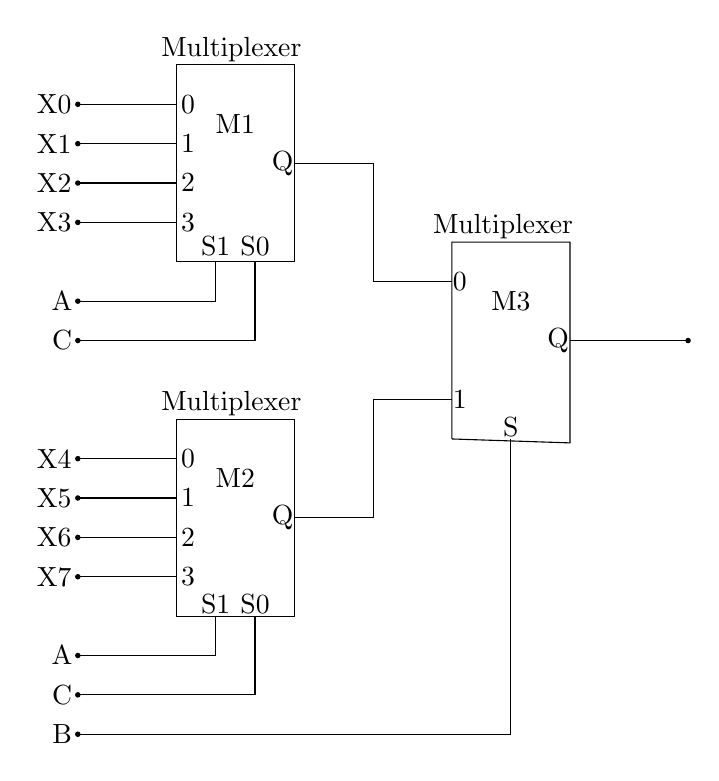
\begin{tikzpicture}[scale=0.5]

%Drawing Multiplexer

\draw (1.4,14.4) node {Multiplexer};
\draw(0,9)--(0,14)--(3,14)--(3,9)--(0,9);
\draw (1.5,12.5) node {M1};
\draw (0.3,10.0) node {3};
\draw (0.3,11.0) node {2};
\draw (0.3,12.0) node {1};
\draw (0.3,13.0) node {0};
\draw (1.0,9.4) node {S1};
\draw (2.0,9.4) node {S0};
\draw (2.7,11.5) node {Q};


\draw (1.4,5.4) node {Multiplexer};
\draw (0,0)--(3,0)--(3,5)--(0,5)--(0,0);
\draw(1.5,3.5) node{M2};
\draw (0.3,1.0) node {3};
\draw (0.3,2.0) node {2};
\draw (0.3,3.0) node {1};
\draw (0.3,4.0) node {0};
\draw (1.0,0.3) node {S1};
\draw (2.0,0.3) node {S0};
\draw (2.7,2.5) node {Q};





\draw (8.3,9.9) node {Multiplexer};
\draw(7.0,4.5)--(7.0,9.5)--(10.0,9.5)--(10.0,4.4)--(7.0,4.5);
\draw (8.5,8.0) node {M3};
\draw (7.2,5.5) node {1};
\draw (7.2,8.5) node {0};
\draw (8.5,4.8) node {S};
\draw (9.7,7.0) node {Q};



%connecting them
\draw (3.0,11.5)--(5.0,11.5)--(5.0,8.5)--(7.0,8.5);
\draw (3.0,2.5)--(5.0,2.5)--(5.0,5.5)--(7.0,5.5);




%connecting clk 
\draw (-2.5,1.0)--(0.0,1.0);
\draw (-2.5,2.0)--(0.0,2.0);
\draw (-2.5,3.0)--(0.0,3.0);
\draw (-2.5,4.0)--(0.0,4.0);
\draw (-2.5,10.0)--(0.0,10.0);
\draw (-2.5,11.0)--(0.0,11.0);
\draw (-2.5,12.0)--(0.0,12.0);
\draw (-2.5,13.0)--(0.0,13.0);
\draw (-2.5,-1.0)--(1.0,-1.0)--(1.0,0.0);
\draw (-2.5,-2.0)--(2.0,-2.0)--(2.0,0.0);
\draw (-2.5,-3.0)--(8.5,-3.0)--(8.5,4.5);
\draw (-2.5,8.0)--(1.0,8.0)--(1.0,9.0);
\draw (-2.5,7.0)--(2.0,7.0)--(2.0,9.0);
\draw (10.0,7.0)--(13.0,7.0);



%drawing clk
\draw (-3.1,1.0) node {X7};
\draw (-3.1,2.0) node {X6};
\draw (-3.1,3.0) node {X5};
\draw (-3.1,4.0) node {X4};
\draw (-3.1,10.0) node {X3};
\draw (-3.1,11.0) node {X2};
\draw (-3.1,12.0) node {X1};
\draw (-3.1,13.0) node {X0};
\draw (-2.9,-1.0) node {A};
\draw (-2.9,-2.0) node {C};
\draw (-2.9,-3.0) node {B};
\draw (-2.9,8.0) node {A};
\draw (-2.9,7.0) node {C};



    % Draw a point at coordinates (-2.5,1.0)
    \fill (-2.5,1.0) circle[radius=2pt];
    % Draw a point at coordinates (-2.5,2.0)
    \fill (-2.5,2.0) circle[radius=2pt];
    % Draw a point at coordinates (-2.5,3.0)
    \fill (-2.5,3.0) circle[radius=2pt];
    % Draw a point at coordinates (-2.5,4.0)
    \fill (-2.5,4.0) circle[radius=2pt];
    

     % Draw a point at coordinates (-2.5,10.0)
    \fill (-2.5,10.0) circle[radius=2pt];
     % Draw a point at coordinates (-2.5,11.0)
    \fill (-2.5,11.0) circle[radius=2pt];
    % Draw a point at coordinates (-2.5,12.0)
    \fill (-2.5,12.0) circle[radius=2pt];
    % Draw a point at coordinates (-2.5,13.0)
    \fill (-2.5,13.0) circle[radius=2pt];


     % Draw a point at coordinates (-2.5,-1.0)
    \fill (-2.5,-1.0) circle[radius=2pt];
     % Draw a point at coordinates (-2.5,-2.0)
    \fill (-2.5,-2.0) circle[radius=2pt];
     % Draw a point at coordinates (-2.5,8.0)
    \fill (-2.5,8.0) circle[radius=2pt];
     % Draw a point at coordinates (-2.5,7.0)
    \fill (-2.5,7.0) circle[radius=2pt];
     % Draw a point at coordinates (13.0,7.0)
    \fill (13.0,7.0) circle[radius=2pt];
     % Draw a point at coordinates (-2.5,-3.0)
    \fill (-2.5,-3.0) circle[radius=2pt];

 
\end{tikzpicture}
\end{figure}
\\
Which one of the following set of values of $(X0, X1, X2, X3, X4, X5, X6, X7)$ will realise the Boolean function 
$\overline{A} + \overline{A}.\overline{C}+A.\overline{B}.C $ ?
 \begin{enumerate}
     \item (1, 1, 0, 0, 1, 1, 1, 0)
     \item (1, 1, 0, 0, 1, 1, 0, 1)
     \item (1, 1, 0, 1, 1, 1, 0, 0)
     \item (0, 0, 1, 1, 0, 1, 1, 1)
 \end{enumerate}

  
\end{enumerate}
\end{document}
